\documentclass{beamer}
\usepackage{beamer}
\usetheme{default}
\usecolortheme{default}
\usepackage[english]{babel}
\usepackage[T1]{fontenc}
\usepackage[utf8]{inputenc} 
\usepackage{graphicx}
\usepackage{filecontents}

\usepackage{tcolorbox}
\tcbuselibrary{fitting}
\usepackage{lipsum}

\tcbset{colframe=blue!50!black,colback=red!10!white,
boxsep=0pt,top=1mm,bottom=1mm,left=1mm,right=1mm,
nobeforeafter,width=\linewidth}


\def\colortheme{dark} % preset themes available are lighten, light, dark
\def\alertcolor{dark} % preset themes available are lighten, light, dark
\setbeamercolor{alerted text}{fg=blue!50!black, bg=white}
\def\upperbar{\true} % i want upper index/navigation bar, \true or \false
\def\bottomsectionbar{\true} % i want bottom bar with Title and Frame/Slide number, \true or \false
\def\bottomtitlebar{\false} % i want bottom bar with Section and Institute, \true or \false

% add bibliography file
\usepackage[backend=biber, style=authortitle]{biblatex}
\addbibresource{bibliography.bib}
\AtBeginBibliography{\small}

\let\Footnotesize=\footnotesize  % save the definition
\let\footnotesize=\tiny  % make a footnotesize change very visible

\setbeamertemplate{footline}

% Add this new command for supervisors/examiners
\newcommand{\supervisors}{
\begin{flushright}
\small
\textbf{Supervisors:} \\
Prof. Claudio Gallicchio,
Dr. Andrea Ceni, 
Dr. Andrea Cossu
}


% % %
\if\upperbar\false
    \setbeamertemplate{headline}{}
\fi
% % %
% set title font smaller
\setbeamerfont{title}{size=\large}
\title[]{Exploring Deep Reservoir Computing
with structured modular architectures}
% make title smaller font


%\subtitle{Subtitle}
%\author{Vincenzo Gargano}
%\supervisors

\author[V. Gargano]{%
\textbf{Author:}\; Vincenzo Gargano\\[0.1em]
\small
\textbf{Supervisors:}\\
Prof.\ Claudio Gallicchio,
Dr.\ Andrea Ceni,
Dr.\ Andrea Cossu
}

\institute
{
  University of Pisa, Deparment of Computer Science. 
}

%\date{\today}

% make date smaller and put it at the bottom of the
% page removing to the center page




\begin{document}

\firstpage % optional. First page

%\indexoverview % optional. Make a slide with index 

\section{Introduction}

% add some space
\begin{frame}
    \centering
    \Large \textbf{Research question:}
    \vspace{1cm}

    \begin{alertblock}{}
        \centering \Large \itshape
        "What is the impact of structured modularities on long short-term memory and learning in reservoir based architectures?"
    \end{alertblock}
\end{frame}
%\sectionoverview % optional. Make a slide with section structure index 
% some background
\begin{frame}{Intro to Reservoir Computing}
    \textbf{Reservoir Computing (RC)} is a paradigm for efficient training of Recurrent Neural Networks (RNNs).
    \newline\newline
    It works as a \textbf{dynamical system} where the reservoir maps inputs into a high-dimensional state space.
    At the same time keeps the Markovian bias of RNNs (ESP).
    \begin{center}
        \includegraphics[width=0.6\textwidth]{images/esn.png}
        \footnote{Image from \href{https://julien-vitay.net/lecturenotes-neurocomputing/4-neurocomputing/4-Reservoir.html}{here}}
    \end{center}
\end{frame}

\begin{frame}{Leaky Echo State Networks}
    \small
    \textbf{Leaky Echo State Networks (ESNs)} have a \textit{fixed}, \textit{randomly connected} reservoir.
    \begin{itemize}
        \item Only the readout is trained (linear regression), ensuring efficiency.
    \end{itemize}
    
    Mathematical formulation of reservoir state update:
    \[
    \mathbf{h}(t) = (1-\alpha)\mathbf{h}(t-1) + \alpha\tanh(\mathbf{W}_{in} \mathbf{u}(t) + \mathbf{W}_{rec} \mathbf{h}(t-1) + \mathbf{b})
    \]
    \small
    where $\mathbf{W}_{in}$/$\mathbf{W}_{rec}$ are input/recurrent weights, $\mathbf{u}(t)$ is input, and $\mathbf{b}$ is bias.
\end{frame}

\begin{frame}{Readout Layer}
    % output layer
The readout layer is a simple linear layer that maps the reservoir state to the output:
\[
y(t) = W_{out} h(t)
\]
It can be easily trained in closed form using ridge regression:
\[
W_{out} = (H^T H + \lambda I)^{-1} H^T Y
\]
where $H$ is the matrix of reservoir states, $Y$ is the matrix of target outputs, and $\lambda$ is a regularization parameter.
\end{frame}

\begin{frame}{Echo State Property (ESP)}
    \small
    For stable dynamics and temporal dependency capture, the \textbf{ESP} must hold for any starting pair $h_{1}(0), h_{2}(0)$:
    \[
    \lim_{t \to \infty} ||h_{1}(t) - h_{2}(t)|| = 0
    \]
    \tiny
    \begin{itemize}    
            \item The reservoir state is uniquely determined by input history, independent of initialization.
            \item \textbf{Condition}: Stability $\mathbf{\rho(W_{rec}) < 1}$ and contractivity $\sigma_{max}(W_{rec}) < 1$. \begin{center}\tcbox{$\rho(A) \leq \sigma_{max}(A)$.}\end{center}
    \end{itemize}
    \tiny
    ESN behave as \textit{"fading memory"} filter over past inputs.

    \begin{center}
        \includegraphics[width=0.95\textwidth]{images/esp.png} % Adjust size as needed
        \footnote{Image from \cite{gallicchio2024euler}}
    \end{center}
\end{frame}

% \begin{frame}{Separation property}
%     % same as esp maybe overkill
% \end{frame}

\begin{frame}{Deep Echo State Networks}
    \begin{columns}
        \begin{column}{0.6\textwidth}
            Adding \textbf{depth} to the reservoir enhances representation capabilities across different time scales, improving performance on complex temporal tasks.
            
            \vspace{1em}
            \textbf{Deep Echo State Networks (DeepESNs)}:
            \begin{itemize}
                \item Progressively filtering of input signal across layers
                \item Preserve ESP over layers 
            \end{itemize}
        \end{column}
        
        \begin{column}{0.4\textwidth}
            \begin{center}
                \includegraphics[width=\textwidth]{../notes/images/modular_deep.png}
                \newline
                \tiny \textit{Stacked Reservoir Architecture}
            \end{center}
        \end{column}
    \end{columns}
\end{frame}

\begin{frame}{Recurrent Oscillatory Networks}
    % maybe add some more details on the architecture
    Recurrent Oscillatory Networks (RONs) are a generalization of Leaky-ESNs, where the reservoir is designed to have oscillatory dynamics.
    \begin{center}
    \includegraphics[width=0.65\textwidth]{images/ron.png}
    \footnote{Credits to \cite{pmlr-v238-ceni24a} for the image}
    \end{center}
\end{frame}

\section{Methodology}

\begin{frame}{Modular Reservoir Computing}
    \begin{columns}
        \begin{column}{0.7\textwidth}
            We introduce the modularity concept on DeepESNs, since they are a specific case of modular architecture.
            
            \vspace{0.5em}
            The reservoir matrix $\mathbf{W_{DeepESN}}$ is block lower-triangular:
            \tiny
            \[
            \mathbf{W_{DeepESN}} = 
            \begin{pmatrix} 
            W_{rec}^{(1)} & 0 & \cdots & 0 \\
            W_{in}^{(2)} & W_{rec}^{(2)} & \cdots & 0 \\
            \vdots & \ddots & \ddots & \vdots \\
            0 & \cdots & W_{in}^{(L)} & W_{rec}^{(L)} 
            \end{pmatrix}
            \]
            \small
            where $W_{rec}^{(l)}$ is the recurrent weight matrix for layer $l$, and $W_{in}^{(l)}$ is the inter-layer weight matrix connecting layer $l-1$ to layer $l$.

        \end{column}
        
        \begin{column}{0.3\textwidth}
            \begin{center}
                \includegraphics[width=\textwidth]{images/layereredres.png}
                \newline
                \tiny \textit{DeepESN as constrained version of shallow reservoir}
            \end{center}
        \end{column}
    \end{columns}
\end{frame}

\begin{frame}{Modular Cycle ESN} % normal itemize, one frame
    \begin{columns}
        \begin{column}{0.35\textwidth}
            \hspace{0.05cm}The \textbf{MC-ESN}, present modules connected in a cycle, and the last layer is connected back to the first one.
        \end{column}
        \begin{column}{0.75\textwidth}
                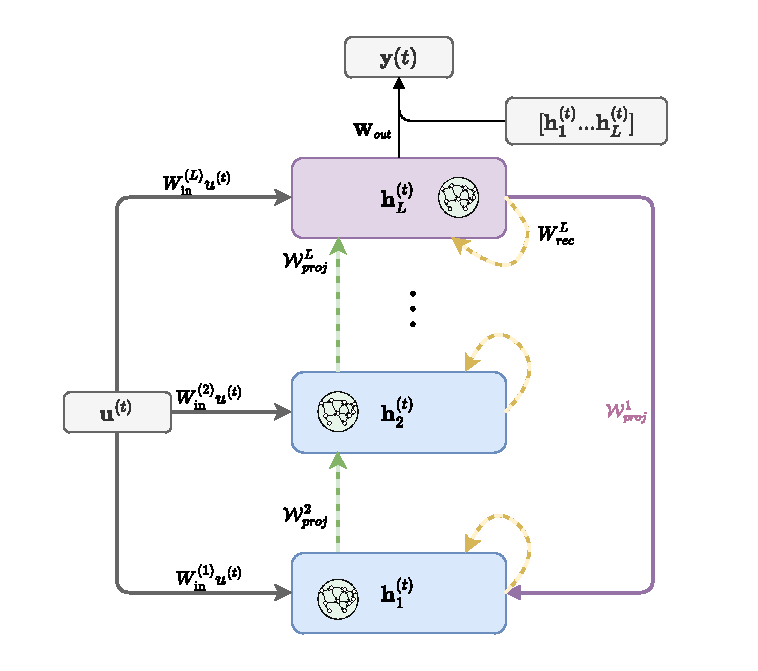
\includegraphics[width=0.85\textwidth]{../notes/images/deep_cycle_reservoir.pdf}
        \end{column}
    \end{columns}
\end{frame}

\begin{frame}{MC-ESN modularity}
    % lower diagonal with W_cyc, top right block W_cyc and the rest is W_rec on diagonal
    The reservoir matrix $\mathbf{W_{MC-ESN}}$ is given by:
        \small
    \[
    \mathbf{W_{MC-ESN}} = \begin{pmatrix}
    W_{rec}^{(1)} & 0 & \cdots & W_{cyc}^{(1)} \\
    W_{cyc}^{(2)} & W_{rec}^{(2)} & \cdots & 0 \\
    \vdots & \ddots & \ddots & \vdots \\
    0 & \cdots & W_{cyc}^{(L)} & W_{rec}^{(L)}
    \end{pmatrix}
    \]
    And the equation for the state update is:
    \tiny
        \begin{equation}
    \begin{aligned}
    \mathbf{h}^{(1)}(t) &= (1-\alpha)\,\mathbf{h}^{(1)}(t-1) \\
    &\quad + \alpha\,\tanh\Big(
    \mathbf{W}_{\text{in}}^{(1)} \mathbf{u}(t)
    + \mathbf{W}_{\text{rec}}^{(1)} \mathbf{h}^{(1)}(t-1)
    + \mathbf{W}_{\text{cyc}}^{(1)} \mathbf{h}^{(L)}(t-1)
    \Big), \\[0.5em]
    \mathbf{h}^{(l)}(t) &= (1-\alpha)\,\mathbf{h}^{(l)}(t-1) \\
    &\quad + \alpha\,\tanh\Big(
    \mathbf{W}_{\text{in}}^{(l)} \mathbf{u}(t)
    + \mathbf{W}_{\text{rec}}^{(l)} \mathbf{h}^{(l)}(t-1)
    + \mathbf{W}_{\text{cyc}}^{(l)} \mathbf{h}^{(l-1)}(t-1)
    \Big).
    \end{aligned}
    \end{equation}
\end{frame}

\begin{frame}{Modular Antisymmetric ESN}
    \begin{columns}
        \begin{column}{0.6\textwidth}
            Another approach is the \textbf{MA-ESN}, with antisymmetric modules across layers..
            
            \vspace{1em}
            We add a constraint on the reservoir weight matrix to enforce antisymmetry:
            \begin{center}
                \alert{Constraint: $C^{(l)} = -C^{(l-1)\top}$}
                \begin{tiny}\footnote{$C^{(l)}$ represents where the signal is projected, in this case from if is the subdiagonal is forwarding toward $l$ from $l-1$, 
                the other way around for upper diagonal skew matrices.}
                \end{tiny}
            \end{center}
            
            \vspace{1em}
            %insert W_{MA-ESN}
            The reservoir matrix $\mathbf{W_{MA-ESN}}$ is given by:
            \tiny
            % tridiagonal with upper diagonal -C^l-1^T and lower diagonal C^l and digonal W_rec^l
        \end{column}
        
        \begin{column}{0.5\textwidth}
            \begin{center}
                \includegraphics[width=\textwidth]{../notes/images/dar.pdf}
            \end{center} 
        \end{column}
    \end{columns}
\end{frame}

\begin{frame}{MA-ESN modularity}

    The reservoir matrix $\mathbf{W_{MA-ESN}}$ is given by:
    % tridiagonal with upper diagonal -C^l-1^T and lower diagonal C^l and digonal W_rec^l
    % color in blue epsilon
    % not use tiny but small
    \small
\[
\mathbf{W_{MA-ESN}} = 
\begin{pmatrix}
W_{rec}^{(1)}-\textcolor[rgb]{0.8,0.6,0.1}{\gamma} I & -\textcolor{blue}{\epsilon} C^{(1)\top} & 0 & \cdots & 0 \\
\textcolor{blue}{\epsilon} C^{(2)} & W_{rec}^{(2)} -\textcolor[rgb]{0.8,0.6,0.1}{\gamma} I & -\textcolor{blue}{\epsilon} C^{(2)\top} & \cdots & 0 \\
0 & \textcolor{blue}{\epsilon} C^{(3)} & W_{rec}^{(3)} -\textcolor[rgb]{0.8,0.6,0.1}{\gamma} I & \cdots & 0 \\
\vdots & \ddots & \ddots & \ddots & -\textcolor{blue}{\epsilon} C^{(L-1)\top} \\
0 & \cdots & 0 & \textcolor{blue}{\epsilon} C^{(L)} & W_{rec}^{(L)} -\textcolor[rgb]{0.8,0.6,0.1}{\gamma} I
\end{pmatrix}
\]
    \tiny
    The state update equations for the Modular Antisymmetric ESN are:
    \begin{equation}
    \label{eq:method:antisym_leak}
    \begin{split}
        \mathbf{h}^{(l)}(t) = (1 - \alpha) \mathbf{h}^{(l)}(t-1) + \alpha \tanh\Bigg( & \underbrace{W_{\text{in}}^{(l)} \mathbf{h}^{(l-1)}(t)}_{\text{Current Input}} \\
        & + \underbrace{(W_{\text{rec}}^{(l)} - \gamma I) \mathbf{h}^{(l)}(t-1)}_{\text{Local Memory}} \\
        & + \underbrace{\epsilon \left( C^{(l)} \mathbf{h}^{(l-1)}(t-1) - C^{\top (l)} \mathbf{h}^{(l+1)}(t-1) \right)}_{\text{Antisymmetric Coupling}} \Bigg)
    \end{split}
    \end{equation}

\end{frame}

\section{Experimental results}

%\sectionoverview % optional. Make a slide with section structure index 

%\subsectionoverview % optional. Make a slide with subsection structure index 

\begin{frame}{Memory Capacity}
Memory Capacity (MC) \footnote{\cite{memorycapacity}} is a measure of how well a RNNs can recall input signal from the past.

Is defined as:
\[MC = \sum_{k=1}^{\infty} \text{corr}^2(y(t-k), \hat{y}(t-k))\]
where $y(t-k)$ is the actual output at time $t-k$ and $\hat{y}(t-k)$ is the output predicted by the network based on its current state.
\end{frame}

%\subsectionoverview % optional. Make a slide with subsection structure index 
\begin{frame}{Memory Capacity results}
    MC-ESN can recover Simple Cycle Reservoirs (SCR)\footnote{\cite{mincomplex}} behaviour, which are known to have maximal $MC\leq N$ where $N$ is the number of neurons in a linear reservoir.
    
    \vspace{1em}
    \begin{columns}
        \begin{column}{0.65\textwidth}
            \centering
            \includegraphics[width=\textwidth]{images/mc_tab.png}
        \end{column}
        
        \begin{column}{0.55\textwidth}
            \centering
            % Placeholder for the second image
            \includegraphics[width=\textwidth]{../notes/images/memory_capacity_vs_delay_esn.png} 
            % Replace 'example-image' with your filename
        \end{column}
    \end{columns}
\end{frame}

\begin{frame}{Long short-term memory}
\small
% insert here
We evaluate the long short-term memory capabilities of the proposed architectures using progressivly complex tasks on 
the MNIST dataset, pixel by pixel, pixel permutation and noise-padded

% add image of mnsit sequential
\begin{center}
    \includegraphics[width=0.65\textwidth]{images/smnist.png}
\end{center}

\end{frame}


\begin{frame}{Results on long short-term memory}
    \small
    Modular Antisymmetric showed improvement in long-term memorization tasks
    \begin{center}
    \includegraphics[width=0.7\textwidth]{images/results_smnist.png}
    \end{center}
\end{frame}
    
\begin{frame}{Results on long short-term memory}
    \small
    \begin{center}
    \includegraphics[width=0.7\textwidth]{images/RESULTSFORD.png}
    \end{center}
\end{frame}

\begin{frame}{Forecasting }
\begin{center}
    \includegraphics[width=0.65\textwidth]{images/RESULTSMG84.png}
\end{center}

\end{frame}


\begin{frame}{Wrap-up and future work}

\small
\begin{itemize}
    \item Modular architectures can enhance memory and learning capabilities of reservoir computing models.
    \item MC-ESN can achieve maximal memory capacity, while MA-ESN shows improved performance on long-term dependencies.
    \item \textbf{Future work}: Eterogeneous layers, more complex modular topologies, small-world and scale-free.
\end{itemize}
\begin{center}
    \includegraphics[width=0.35\textwidth]{../proposalphd/modular.pdf}
\end{center}

\end{frame}


% add references
\begin{frame}[allowframebreaks]{References}
    \printbibliography
\end{frame}

\begin{frame}
    % thank you
    \begin{center}
        \Large \textbf{Thank you!}
    \end{center}
\end{frame}


%\appendix % appendix
\begin{frame}{Supporting Materials: Eigenvalues distributions MC-ESN and MA-ESN}
    %% add plot of eigenvalues distribution of jacobians
    We present three settings: a contractive, one showing violation of ESP and last showing edge of stability.
    \begin{center}
    \includegraphics[width=0.85\textwidth]{images/cycle_eigenvalues_distirbution.png}
    \end{center}
    \begin{center}
    \includegraphics[width=0.9\textwidth]{images/eigenvalue_distributions_esn_antisym.png}
    \end{center}
\end{frame}


\begin{frame}{Supporting Materials: Reservoir states differences (DeepESN)}
    \begin{center}
    \includegraphics[width=0.9\textwidth]{images/distance_reservoir_states_DeepReservoir_5_layers.png}
    \end{center}
    %% add plot of eigenvalues distribution of jacobians
\end{frame}

\begin{frame}{Supporting Materials: Reservoir states differences (MC-ESN)}
    \begin{center}
    \includegraphics[width=0.9\textwidth]{images/distance_reservoir_states_Cycle DeepReservoir_5_layers.png}
    \end{center}
    %% add plot of eigenvalues distribution of jacobians
\end{frame}
\begin{frame}{Supporting Materials: Reservoir states differences (MA-ESN)}
    \begin{center}
    \includegraphics[width=0.9\textwidth]{images/distance_reservoir_states_Antisymmetric DeepReservoir_5_layers.png}
    \end{center}
    %% add plot of eigenvalues distribution of jacobians
\end{frame}
    
\end{document}

